\documentclass[11pt]{article}
\usepackage{fontspec}
\usepackage{graphicx}
\usepackage{diagbox}
\usepackage{amsmath,bm}
\usepackage{caption}
\usepackage{subcaption}
\usepackage{hyperref}
\usepackage[capitalise,noabbrev]{cleveref}
\setmainfont{Arial}
\usepackage{setspace}

\doublespacing
\usepackage{geometry}
 \geometry{
 a4paper,
 total={170mm,257mm},
 left=20mm,
 top=20mm,
 }
\usepackage{amsmath}

\begin{document}

% Chapter2
\tocdata{toc}{Di Wan}



\chapter{Product Design} % Main chapter title

\label{Chapter2} % Change X to a consecutive number; for referencing this chapter elsewhere, use \ref{ChapterX}

\section{Introduction}
App design combines User interface (UI) and User Experience (UX); while UI is concerned about how the app pages look and feel, such as the fonts, colours and arrangements of icons, UX focuses on the functionality and usability. The primary goal of any business is to increase its sales and push the growth of the business, and UX/UI Design plays an essential role in achieving this goal. It's the primary reason companies keep updating their apps. Currently, we only focus on the mobile app design or specifically IOS design (based on Apple Platform) and Android Design, because of limited project time length.
%-----------------------------------------------------------------------------------------------------------------------------UX
\section{UX Design}
UX Design decides how someone will use an app and create a viable product. During the UX process, mobile app design ideas are generated and validated to ensure that all choices will work so that our app works. The quality of the user experience is the crucial factor in measuring the quality of the design. Usually, it is the key to distinguishing a successful app design from an unsuccessful one. Customers are becoming pickier about which app to use and so quick to abandon the app they do not enjoy, so investing time and effort in creating a great user experience is essential. Also, a study by UXERIA shows that 70\% of online businesses fail because of lousy usability\footnote{Doris Wójcicka UX designer, Wójcicka, D., &amp; designer, U. X. (2015, November 21). 15 statistics that will convince your boss to invest in UX! Uxeria Blog. Retrieved May 15, 2022, from https://blog.uxeria.com/15-statistics-that-will-convince-your-boss-to-invest-in-ux/ }, so we need to consider carefully about the user experience throughout the development process.
\subsection{Minimum Viable Product (MVP)}
A minimum viable product or MVP is a product with enough features to attract early-adopter customers and validate a product idea early in the development cycle.\footnote{Minimum viable product (MVP). ProductPlan. (2021, August 12). Retrieved May 15, 2022, from https://www.productplan.com/glossary/minimum-viable-product/} 
To decide which parts belong to the MVP design, we use the MoSCoW method introduced by Software development expert Dai Clegg to represent all the features we want to include in our design. It is a popular prioritization technique for managing requirements and the acronym MoSCoW represents four categories of initiatives: must-have, should-have, could-have, won’t-have, or will not have right now.\footnote{Moscow prioritization. ProductPlan. (2021, September 10). Retrieved May 15, 2022, from https://www.productplan.com/glossary/moscow-prioritization/}
The table separates the features for our MVP from the advanced functions that we want to include in our design, and the MoSCoW table for our design can be seen in \cref{moscow}.

\begin{table}[ht]
\centering
\begin{tabular}{ |c|c| } 
 \hline
\textbf{MUST-HAVE FEATURES FOR MVP} & \textbf{SHOULD/ COULD HAVE FEATURES}\\ 
 \hline
 Sign-up and sign-in with email & Sign-in with third party accounts \\ 
 \hline
 Upload Audio & Real-time generation \\ 
 \hline
 Chord output & Chord regeneration \\ 
 \hline
 Chord layout &  Export to PDF \\ 
 \hline
 Share posts & Message channel \\ 
 \hline
 Recommendation Engine &  Lock Chords when regenerating\\ 
 \hline
 Help and support &  Pitch Tracking\\ 
 \hline
 File storage& File backup \\ 
  \hline
 & Mood Classification \\ 
  \hline
 & Shifting key \\ 
 \hline
 \end{tabular}
 \caption{MoSCoW Table}
 \centering
 \label{moscow}
 \end{table}
 
 \subsection{Main Function Explained}

\begin{itemize}

\item \textbf{Sign-up and Sign-in with Email}
\\From the start, our users can sign up with their email and log in with our app accounts. We want our users to create an account so that we can profile our users more easily.

\item \textbf{Sign-in with third-party Accounts}
\\ The purpose is to reduce our users' barriers to entering our app. OAuth (Open Authorisation)\footnote{Auth0. (n.d.). Authentication - reduce risks and remove barriers. Auth0. Retrieved May 15, 2022, from https://auth0.com/authentication } is an open standard for access delegation, and it is commonly used for internet users to grant websites or applications access to their information on other websites without giving them the passwords. We will include OAuth in our design to allow our users to sign in with Facebook and Google accounts since those are the most common social media accounts people have.

\item \textbf{Ask for song tag preference}
\\After our users sign in, they will be asked about the feature preferences, and we provide limited choices of answers they can choose from. The answers will be stored and fed to our recommendation engine (\cref{Content Based Recommendation System}). 

\item \textbf{Store and backup files on Cloud}
\\The purpose is to enable better synchronisation between devices and accessibility to the files. Since developing our own cloud drive is time-consuming and less secure than directly combining the existing cloud platform into our design. 
We will include CloudKit\footnote{Inc., A. (n.d.). CloudKit - icloud. Apple Developer. Retrieved May 16, 2022, from https://developer.apple.com/icloud/cloudkit/} in our IOS design to allow users to store their saved files in iCloud. Also, we will enable users to save files on Google Drive by using Google Drive API.

\item \textbf{Recording input}
\\ To obtain the audio source, we allow our users to record their singing using our app or upload a previous recording 
from a built-in app such as Voice Memos on iPhone. For ethical reasons (\cref{sec:dataethics}), we will ask permission first to access the microphone and recording apps.

\item \textbf{Chord generation and regeneration}
\\Unlike Chordify, which generates the same chords each time for the same audio source, we provide the option for users to regenerate the chords. We aim to provide sightly different chords when the regeneration button is pressed. 
We will also allow our users to lock the chords they like during the regeneration. The theory behind it will be introduced in \cref{Ed part}.

\item \textbf{Community Page}
\\Inspired by the Chinese music app NetEase, one of our goals is to create a community page for our users to share their works and collaborate, 
we believe that the community element can bring continuous traffic to our app, which can benefit the monetisation of our app in the future.
As we mentioned before, the user experience determines the success of the app design. Here, the quality of the posts recommended to our users is an essential element affecting our user experience. 
Therefore, it requires our recommendation engine to be well-designed. (\cref{Chapter6})

\item \textbf{Message Channel}
\\The message channel allows our users to contact each other directly and share the original chord files to collaborate on. For privacy reasons, we design our message system using end-to-end encryption to protect the content in the conversation from tapping.

\end{itemize}

\subsection{User Flow}
 \textbf{User flows} are flowcharts that illustrate the movement or journey of a user through the app. User flow diagrams are indispensable in mastering user experience. 
 They allow us to understand how users interact with our app and their steps to complete a task or achieve a goal on our app, 
 which will help us create a superior user experience for the user and meet their needs more efficiently. 
 \\One of our user flow examples is shown in \cref{flowchartmain}
 We use rounded rectangles to represent the terminations, diamonds to represent the decisions, rectangles to represent the processes, and arrows to represent the flow directions.

\begin{figure}[ht]
\centering
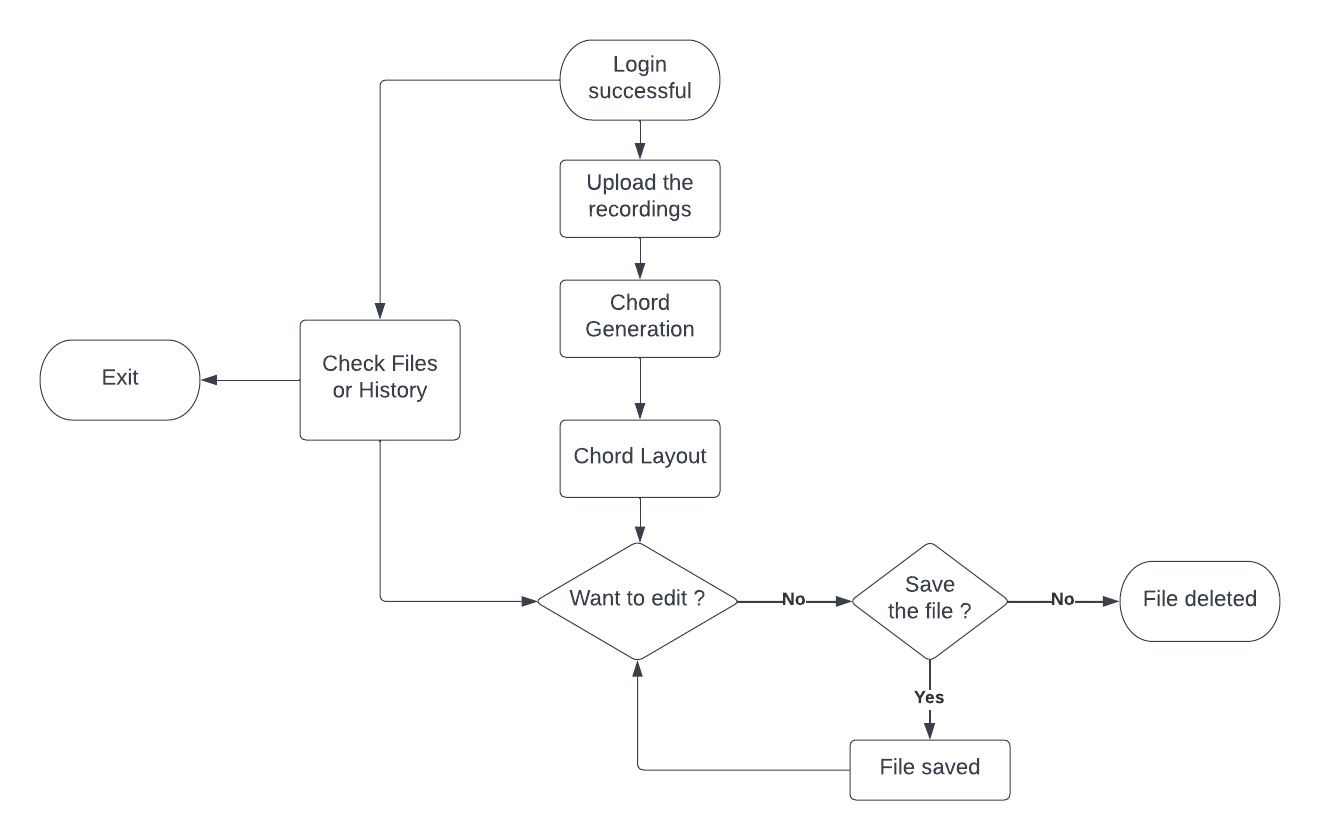
\includegraphics[scale = 0.25]{MFpage.png}
\caption{User Flow Diagram for main function page}
\label{flowchartmain}
\end{figure}
%-----------------------------------------------------------------------------------------------------------------------------UI
\section{UI Design}
After having all the user flow maps of our design, we started to design the prototype using Figma, a design tool for prototyping projects. 
There are three example sketches in \cref{fig:UIdesign}. 

\begin{figure}[ht]
     \centering
     \hspace{16mm}
     \begin{subfigure}[b]{0.2\textwidth}
         \centering
         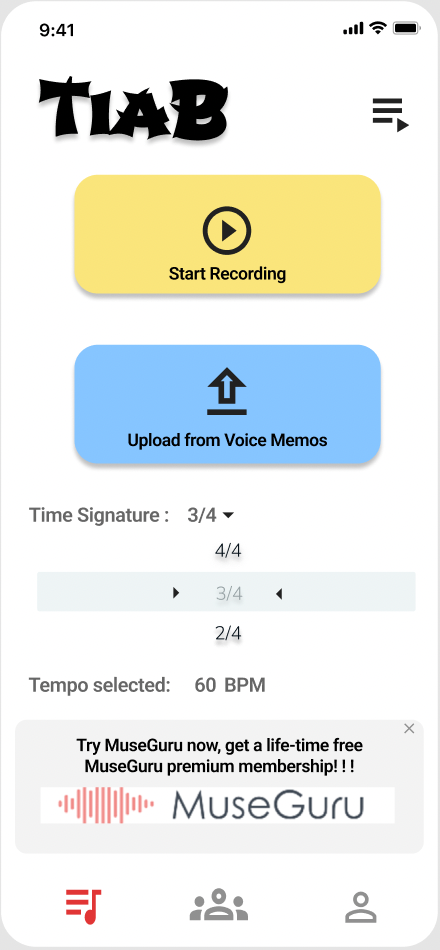
\includegraphics[width=\textwidth]{mianpage1.png}
         \caption{Main page - audio-upload page}
         \label{Mainpage}
     \end{subfigure}
     \hfill
     \begin{subfigure}[b]{0.2\textwidth}
         \centering
         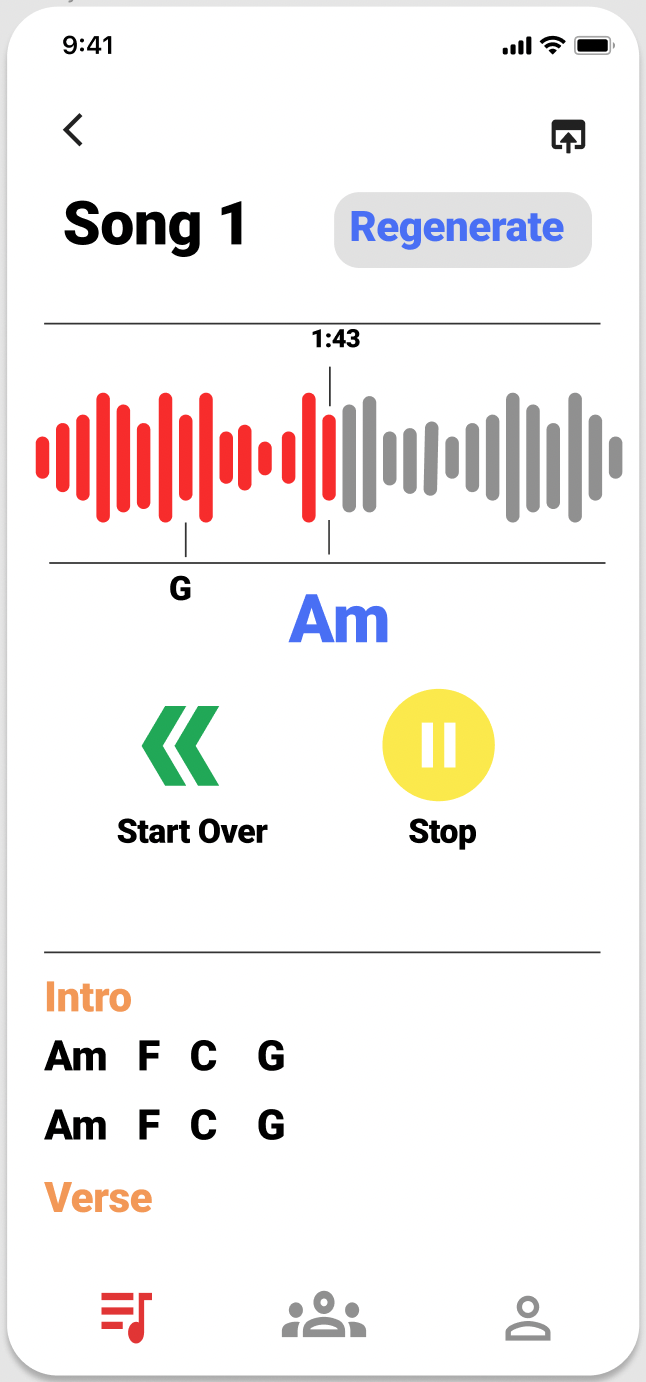
\includegraphics[width=\textwidth]{grappp.png}
         \caption{Chord layout and editing page}
         \label{chordedit}
     \end{subfigure}
     \hfill
     \begin{subfigure}[b]{0.2\textwidth}
         \centering
         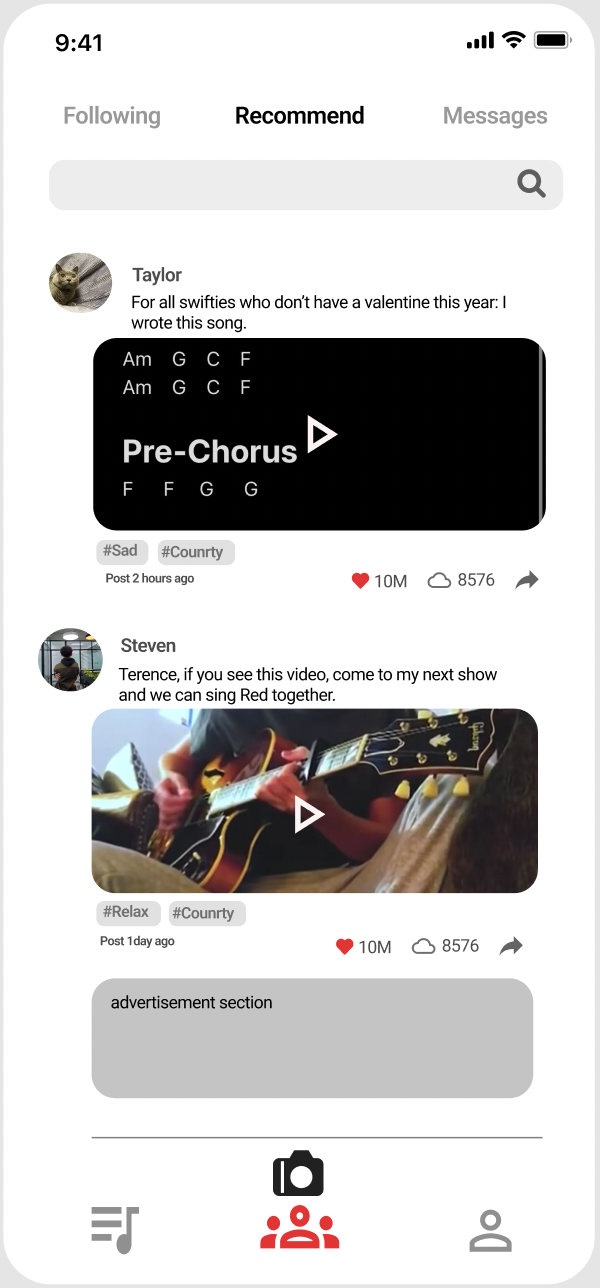
\includegraphics[width=\textwidth]{commupage.png}
         \caption{Community page}
         \label{Community page}
     \end{subfigure}
     \hspace{16mm}
        \caption{UI design for our app}
        \label{fig:UIdesign}
\end{figure}


\section{Testing}
\label{ch2test}
The testing stage allows us to discover the problems in our current designs and improve our existing designs. 
According to Compuware, 48\% of users are less likely to use an app again if they are troubled with its performance.
As reported by Compuware, only 16\% of users can give the app a try for a second or third time.\footnote{Perez, S. (2013, March 12). Users have a low tolerance for buggy apps – only 16\% will try a failing app more than twice. TechCrunch. Retrieved May 15, 2022, from https://techcrunch.com/2013/03/12/users-have-low-tolerance-for-buggy-apps-only-16-will-try-a-failing-app-more-than-twice/?} Hence it is essential for 
\\We divide our testing stage into four stages, Unit Tests, Integration Tests, System Tests, and Acceptance Tests.
\begin{itemize}
\item\textbf{Unit Test} is the very first stage of any application test. At this step, the system’s separate modules will undergo assessments to see if they individually function correctly to maximum capacity. 
\item\textbf{Integration Test} is mostly about verifying the modules and examinating their readiness and collective and integral cooperation. The modules are each tested separately and also as a group. It helps the testers identify any issues with two or more components working together or individually to execute functions.
\item\textbf{System Test} level closely simulates the final production environment. It is very significant in the final testing stage, especially when it needs to ensure that the applications under scrutiny always meet complete functional requirements. 
At this stage, the test team ascertains if the integrated components are collectively showing optimal performance levels or not. Every software build must undergo testing up to this point, using client requirements as a benchmark. This stage is carried out by the quality assurance engineer in our team.
\item\textbf{Acceptance Test} is the stage where we will use A/B testing to understand how users respond to our design. 
A/B testing is a method of comparing two versions of a webpage or app against each other to determine which one performs better.\footnote{A/B testing. Optimizely. (n.d.). Retrieved May 16, 2022, from https://www.optimizely.com/optimization-glossary/ab-testing/} It is an essential experiment where two or more variants of a design are shown to users at random. Based on the statistical analysis, we can determine which variation performs better for a given conversion goal.
After we have a functionally-reliable version of the app, 
we will be performing A/B testing by providing different UI designs to other groups of test users. This method allows us to 
determine which option is more attractive.\end{itemize}

\section{Summary}
In the chapter, we discussed the minimum viable product of our design and demonstrated the critical steps throughout our design process. For each function we want to include in our design, we also showed the essential components that must be contained to achieve full functionality. We could not finish the app's programming because of the limited project time, high complexity, and time-consuming coding process. However, we explained how we would perform the testing stage in the future if we had our MVP.

\end{document}
